\documentclass[12pt,a4paper]{report}

\usepackage[utf8]{inputenc}
\usepackage{relazione}

\title{Mambelli Domain Model - Project Management}
\author{
  Giacomo Cavalieri \\ \emailaddr{giacomo.cavalieri2@studio.unibo.it}
  \and
  Nicolò Di Domenico \\ \emailaddr{nicolo.didomenico@studio.unibo.it}
  \and
  Linda Vitali \\ \emailaddr{linda.vitali2@studio.unibo.it}
}
\date{\today}

\begin{document}

\maketitle

\newpage
\tableofcontents
\newpage
\listoftodos
\newpage

\chapter*{Introduzione}

\emph{Mambelli Domain Model} è un progetto realizzato per il corso di Laboratorio di Sistemi Software.
Il progetto è stato sviluppato da un \href{https://atedeg.dev/about}{gruppo di quattro studenti} per l'azienda cesenate \emph{Mambelli} che si occupa di produzione e vendita di prodotti caseari.

Le modalità di acquisizione dei requisiti, di interazione coi committenti e l'organizzazione tramite metodologia \emph{Agile} riportate nel seguente documento sono state effettivamente impiegate dai membri del gruppo nella realizzazione del progetto. Tuttavia, ai fini dell'esame di \emph{project management} si è immaginato che il team fosse composto da più membri di quanto non fosse in realtà, per poter mettere in luce in maniera più efficace i diversi concetti appresi di project management.

Il progetto è stato sviluppato secondo la metodologia del \emph{Domain Driven Design}~\cite{cit:ddd} facendo ampio uso di \emph{Event Storming}~\cite{cit:event-storming} per gestire la comunicazione con i committenti e la raccolta dei requisiti.

Questo documento contiene tutte le informazioni relative ai processi di project management messi in atto per la gestione del progetto. Inoltre, in appendice sono inclusi tutti i diversi documenti prodotti.
La documentazione tecnica può invece essere consultata all'apposito \href{https://atedeg.dev/mdm/_docs/introduction.html}{sito web}.

\chapter{Scoping}\label{ch:scoping}

- [X] introduzione
- [X] chi siamo
- [X] chi sono i committenti
- [X] richiesta del cliente
  - [X] i loro problemi che vogliono risolvere
- [ ] analisi del dominio (meeting fatti)
  - [ ] event storming
- [ ] user stories  
- [ ] POS 


\section{Profilo della software house}\label{sec:profilo-della-software-house}
Atedeg è una software house che opera sul territorio cesenate. È composta da un team piuttosto affiatato di 10 persone dalle competenze più variegate, che si occupano di sviluppo software.

Il core team è composto da Giacomo, Linda, Nicolas e Nicolò, quattro amici che si sono conosciuti all'università e hanno deciso, una volta terminati gli studi, di fondare la software house.
Nel corso degli anni, il team si è arricchito di nuovi membri, che hanno portato con sé nuove idee e hanno contribuito a mantenere Atedeg un ambiente dinamico aperto all'innovazione. 

Essendo una piccola software house, Atedeg non adotta una rigida suddivisione gerarchica dei ruoli. In particolare, non esiste un senior management che decida quali progetti intraprendere o meno: infatti, tali decisioni vengono prese in comune dai membri del team, che si riuniscono periodicamente per discutere di nuovi possibili progetti. In questo modo, tutti i colleghi hanno la possibilità di esprimere le proprie opinioni e di partecipare attivamente alla vita dell'azienda.

All'interno di Atedeg si dà molta importanza all'arricchimento personale e professionale, e si cerca di dare a tutti gli sviluppatori la possibilità di crescere e di migliorare le proprie competenze. Per questo motivo sono incentivati lo studio e la formazione e, qualora i dipendenti ne facciano richiesta, l'azienda cerca di finanziare la loro partecipazione a conferenze di calibro internazionale. \todo[inline]{Mettere nella organizzazione delle ore il fatto che uno dei membri deve andare a una conferenza a Zurigo per tre giorni} In particolare, Linda ha avuto modo di assistere al ciclo di conferenze \href{https://dddeurope.com}{\emph{Domain Driven Design Europe}} del 2019 e da quel momento ha cercato di introdurre gradualmente nell'azienda il Domain Driven Design, che è stato adottato in due progetti conclusi con successo.

\section{Profilo del committente}\label{sec:profilo-del-committente}
Mambelli è un caseificio di Cesena a gestione familiare che si occupa di produzione e vendita di prodotti caseari. L'azienda è stata fondata nel 1972 e nel corso degli anni si è arricchita di nuove produzioni ricevendo anche diversi riconoscimenti come il premio \emph{Italian Cheese Award}. 
Grazie alla crescente popolarità è aumentata anche la domanda di prodotti e, per poterla soddisfare, Mambelli ha deciso di migliorare il proprio sistema informativo automatizzando, laddove possibile, i diversi processi aziendali.

L'azienda è gestita da Raffaella che si occupa dell'acquisto delle materie prime e della pianificazione della produzione dei formaggi. Il marito di Raffaella, Gianluca, si occupa invece dei rapporti coi clienti e della gestione degli ordini. Inoltre il caseificio assume due casari che si occupano della produzione dei formaggi e del controllo qualità dei prodotti. Infine l'azienda ha diversi dipendenti impiegati nel settore della logistica.

\section{Richiesta del committente}\label{sec:richiesta-del-committente}
L'attuale sistema informativo adottato dal caseificio Mambelli risulta inadeguato per poter gestire l'aumento nella domanda dei prodotti: molti dei processi aziendali sono infatti gestiti manualmente o su semplici fogli elettronici.
\begin{itemize}
  \item \textbf{Gestione degli ordini:} al momento tutti gli ordini arrivano tramite mail o, in maniera informale, tramite comunicazioni telefoniche. Gianluca impiega quindi molto tempo per raccoglierli e inserirli nel sistema informativo. Inoltre, non essendo strutturati, gli ordini non sono facilmente consultabili e non è possibile ricavare informazioni utili per la pianificazione della produzione
  \item \textbf{Pianificazione della produzione:} la pianificazione di quali prodotti mandare in produzione viene fatta manualmente da Raffaella sulla base della sua grande esperienza nel campo. Per prendere queste decisioni Raffaella consulta un foglio elettronico che riporta alcune informazioni sugli ordini passati e su quanto è stato prodotto in precedenza. Sebbene questo metodo sia sufficiente per poter effettuare la programmazione, presenta due importanti problemi:
  \begin{itemize}
    \item Raffaella, grazie alla sua esperienza, è l'unica in grado di pianificare la produzione; se dovesse essere assente per qualche motivo, la produzione non potrebbe essere pianificata in maniera adeguata
    \item Sebbene l'esperienza di Raffaella sia sufficiente per avere delle buone pianificazioni, queste potrebbero essere ottimizzate ulteriormente con il supporto di sistemi informativi più avanzati riducendo i tempi morti nell'uso dei macchinari e minimizzando gli sprechi di materie prime
  \end{itemize}
\end{itemize}
\todo[inline]{Far vedere che nelle riunioni emergono ulteriori pain point: integrazione col sistema della tracciabilità, etc.}
\todo[inline]{Possibile rischio è che i clienti non apprezzino il nuovo sistema per gli ordini, mitigazioni che possiamo adottare: 
User Experience e incontri con persone per farglielo provare, suggerimento all'azienda di mettere sconti inizialmente per chi fa gli ordini online, NLP che estrae dalla mail il contenuto dell'ordine (questo però introduce ulteriori rischi)}


\chapter{Planning}\label{ch:planning}

\section{Joint Project Planning Session}\label{sec:JPPS}
Complessivamente si sono svolte tre riunioni di \emph{Joint Project Planning} con il committente. In seguito sono riportati i partecipanti delle riunioni e ciò che è stato deciso opportunamente motivato.

\subsection{Partecipanti}
\begin{itemize}
  \item I membri del core team di Atedeg che hanno già preso parte alle riunioni precedenti: Giacomo, Linda (facilitatore e product owner), Nicolas e Nicolò
  \item Un altro sviluppatore di Atedeg
  \item Raffaella (project sponsor e process owner dei processi relativi alla pianificazione della produzione)
  \item Gianluca (process owner dei processi aziendali relativi a gestione ordini e magazzino)
  \item Simone (process owner dei processi aziendali relativi alla produzione)
\end{itemize}

\subsection{Kick-off}
La prima riunione si avvia con la presentazione dei partecipanti e un breve riassunto di quanto discusso nelle riunioni precedenti. In particolare Raffaella ha spiegato come il progetto si inserisce nella strategia aziendale e quali sono gli obiettivi che si prefigge: efficientare il processo di gestione degli ordini e automatizzare la pianificazione della produzione aumentando la produttività dei macchinari del caseificio.
Dopodiché è avvenuta la presentazione del team di Atedeg.

\subsection{Working session}

\subsubsection{Validazione e panoramica dell'approccio scelto}
Come già discusso nella precedente riunione, il team ha deciso di adottare un approccio di sviluppo Agile con metodologia Scrum. La scelta è stata discussa e approvata con il committente che si è reso disponibile a prendere parte alle riunioni di \emph{sprint review}.

Di comune accordo si è stabilito che la durata di ogni sprint fosse di due settimane e che le riunioni di review si tenessero di lunedì. Infine è stato deciso che la \emph{product owner} sarebbe stata Linda, che ha già esperienza sia con la metodologia Scrum che con lo sviluppo DDD.

\subsubsection{Validazione e prioritizzazione dei requisiti}
Per quanto riguarda i requisiti, il team ha deciso di assegnare insieme al committente una priorità numerica da 1 (la più bassa) a 5 (la più alta) a ciascuna epica.
La stessa scala di priorità è stata usata anche per prioritizzare le user story all'interno della loro rispettiva epoca.
Vista l'esigenza del committente di avere un sistema (anche minimo) che permettesse di raccogliere e gestire gli ordini entro settembre, si è deciso di comune accordo di dare la massima priorità all'epica \href{user-story:i2-e4}{I2-E4}, con le altre correlate a seguire.

\subsubsection{Stima delle risorse}
La quantità di lavoro di ciascuna user story è stata stimata assegnandovi un valore scalare adimensionale: gli \emph{story points}.
Per assegnare gli story points è stato usato il metodo \emph{Delphi}: questa tecnica consiste nel chiedere a ciascun membro del team di stimare la quantità di lavoro di una user story, e poi di fare dei nuovi round tenendo conto delle stime e motivazioni degli altri membri del team. Questo procedimento viene ripetuto finché non si converge a un risultato comune o non si raggiunge un numero di round prefissato.
In caso di mancata convergenza, si è deciso di usare la media delle stime come valore finale.

Indicativamente un punteggio di 5-6 story points indica una user story semplice che può essere completata in un paio di giornate lavorative, mentre un punteggio superiore indica user story più complesse che potenzialmente potrebbero richiedere anche l'intero sprint; un esempio di tale user story è la \href{user-story:i1-e1-u1}{I1-E1-U1}.

Una volta stimata la complessità delle user stories è stata adottata nuovamente la Delphi technique per stimare il numero di persone ideale da assegnare a ciascuna storia. Per farlo si è tenuto in considerazione quanto ciascun task potesse essere parallelizzabile cercando di assegnare più sviluppatori a user story complesse.

Infine, non è stato immediatamente realizzato il \emph{project network diagram} per non imporre una linearizzazione nello sviluppo del progetto che essenzialmente avrebbe fatto perdere i vantaggi nell'utilizzare Scrum. Per questo motivo, si è stabilito di realizzare uno \emph{sprint network diagram} all'inizio di ciascuno sprint per poter permettere al project manager di pianificare al meglio l'uso delle risorse e dei tempi al suo interno.

\subsubsection{Analisi dei rischi}
In seguito sono stati analizzati in dettaglio i rischi riportati nel POS; in particolare, per ciascuno è stata stabilità la probabilità che si verifichi, l'impatto ed eventuali strategie di mitigazione. Il documento risultante è riportato in \Cref{app:analisi-rischi}.

\subsubsection{Gestione del cash flow}
Per stimare i costi del progetto il team fa affidamento alla propria esperienza con progetti passati. Infatti, avendo già esperienza con la realizzazione di portali e-commerce e gestionali il team ha stimato di poter concludere il progetto in 4 sprint di due settimane ciascuno. D'altro canto la porzione relativa all'integrazione e alla pianificazione della produzione rappresentano la complessità maggiore e si è stimato che possano impiegare 2 interi sprint. 
Quindi, nelle stime riportate al cliente viene data come durata indicativa del progetto 6 sprint, rendendo comunque chiaro il fatto che il progetto potrebbe richiedere più tempo per essere terminato.

Ogni dipendente di Atedeg viene pagato \EUR{25} l'ora e la settimana lavorativa è di 32 ore. Per terminare il progetto nei limiti prestabiliti si è scelto di assegnarvi 5 sviluppatori full-time. Dunque, ciascuno sprint avrà un costo di \EUR{8\,500} (tenendo conto anche dei costi delle utenze e delle licenze software) e il progetto complessivamente potrebbe costare indicativamente \EUR{51\,000}.

Il committente ha accettato il progetto con un contratto a corpo dove, al termine di ogni sprint di due settimane viene corrisposta la cifra di \EUR{8\,500}.
Inoltre, il committente ha accettato di pagare un anticipo di \EUR{4\,000} per coprire i costi di avvio del progetto.

\chapter{Launching}\label{ch:launching}

\section{Staffing}\label{sec:staffing}

Nella fase di planning si è stimato essere necessario avere 5 sviluppatori full-time per completare il progetto. Per questo motivo, il team che ha preso parte alla fase di planning corrisponde con il developer team: Asia, Giacomo, Linda (che ha anche ricoperto il ruolo di product owner), Nicolas e Nicolò.
Tutti i membri del team hanno già grande esperienza con progetti Scrum, per questo motivo non è stato necessario ingaggiare uno Scrum Master che guidi il team nell'applicazione di questa metodologia.

I membri del team sono ``persone fatte a T'': con questo termine si indica una persona con capacità di comprendere e affrontare uno spettro ampio di temi e problematiche -- rappresentato dalla barra orizzontale della T -- e allo stesso tempo con una forte competenza in una specifica materia -- rappresentata dalla barra verticale. Questo permette al team di avere una grande varietà di competenze e di poter affrontare qualsiasi problema che si presenti durante lo sviluppo del progetto. In seguito sono riportati i punti di forza di ciascuno sviluppatore:
\begin{itemize}
  \item Asia (\emph{accommodating}): ha grande esperienza nello sviluppo frontend, di interfacce utente con particolare attenzione alla user experience
  \item Giacomo (\emph{assimilating}): è esperto nella realizzazione di sistemi basati su una architettura funzionale e in linguaggi di programmazione funzionali 
  \item Linda (\emph{accommodating}): è esperta di Domain Driven Design e di modellazione di domini complessi
  \item Nicolas (\emph{diverging}): ha grande esperienza nell'utilizzare pratiche agili e strumenti automatizzati per garantire la qualità del codice, la scalabilità del sistema e la sicurezza delle operazioni
  \item Nicolò (\emph{converging}): è esperto nella progettazione, training e valutazione di sistemi di machine learning
\end{itemize}

\todo[inlne]{BOH sta croce non va}
\begin{figure}
  \centering
  
\begin{tikzpicture}
    \draw[line width=30pt] (0,0) -- (0,6) node [midway, rotate=90] {conoscenze};  % linea verticale
    \draw[line width=30pt] (-3,3) -- (3,3) node[midway] {competenze}; % linea orizzontale
  \end{tikzpicture}
  \caption{Persona a T}
  \label{fig:croce}
\end{figure}

\todo[inline]{Decidere se fare o meno il Project Definition Statement}

\section{Definizione delle regole operative}
\subsection{Project meeting}
È stata definita la gamma di possibili meeting a cui il team dovrà partecipare, la loro durata e cadenza.

\subsubsection{Standup meeting}
Gli \emph{standup meeting} si svolgono con cadenza giornaliera e non impiegano più di 10 minuti. Questi meeting coinvolgono tutti i membri in piedi ogni mattina prima di iniziare la giornata.
Questi si svolgono in maniera informale e non hanno una scaletta esplicita: i membri del team di sviluppo discutono su ciò che stanno facendo e presentano gli eventuali problemi riscontrati. 
Nel caso in cui siano presenti problemi che impediscano di proseguire con lo sviluppo, il team si riunirà in un \emph{problem resolution meeting} per discutere più nel dettaglio del problema.

\subsubsection{Problem Resolution Meeting}
I problem resolution meeting vengono indetti in maniera straordinaria qualora durante uno standup meeting emerga un problema grave. Alla riunione partecipano il product owner, il \emph{problem owner} ed eventuali sviluppatori che possono essere affetti dal problema. Le riunioni si svolgono secondo una scaletta predefinita:
\begin{itemize}
  \item Vengono raccolte informazioni sul problema
  \item Si cercano possibili soluzioni tramite \emph{brainstorming}
  \item I partecipanti si consultano per decidere la soluzione migliore; nel caso in cui sia necessario potrebbero essere interpellati anche altri membri del team per chiedere un loro parere
  \item Si aggiorna lo \emph{sprint backlog} in modo da includere i task necessari a implementare la soluzione scelta al problema
\end{itemize}

\subsubsection{Sprint review}

\subsubsection{Sprint retrospective}

\subsubsection{Sprint planning}



\chapter{Monitoraggio e controllo}
\label{ch:monitoraggio-e-controllo}

Il progetto è stato gestito col supporto di \emph{GitHub Projects}~\cite{cit:github-projects}. Questo strumento si integra con il DVCS Git utilizzato dal team e permette di gestire le attività di sviluppo in modo agile.
Inoltre, è stata prestata grande attenzione ad automatizzare il più possibile queste attività per ridurre al minimo il tempo necessario per la loro esecuzione e permettere agli sviluppatori di concentrarsi sui problemi di business.

\section{Reporting automatico}
\label{sec:reporting-automatico}

Ogni task dello sprint viene convertito in una GitHub issue~\cite{cit:github-issues} che ne riporta le dipendenze e le informazioni di base; un esempio di tale issue è riportato in \Cref{fig:issue-example}. Come mostrato in figura, il vantaggio di tale approccio sta nella possibilità di automatizzare il reporting delle attività svolte durante lo sprint. Infatti, un bot può analizzare le dipendenze fra task -- ricostruendo così lo sprint network diagram --, calcolare il percorso critico e notificare gli sviluppatori di eventuali ritardi.

Grazie alla stretta integrazione fra il sistema di reporting e il DVCS, il programmatore non dovrà occuparsi di gestire alcun overhead dato che gli sarà sufficiente chiudere una issue per segnalare che il task corrispondente è stato completato.

\begin{figure}[htp]
  \centering
  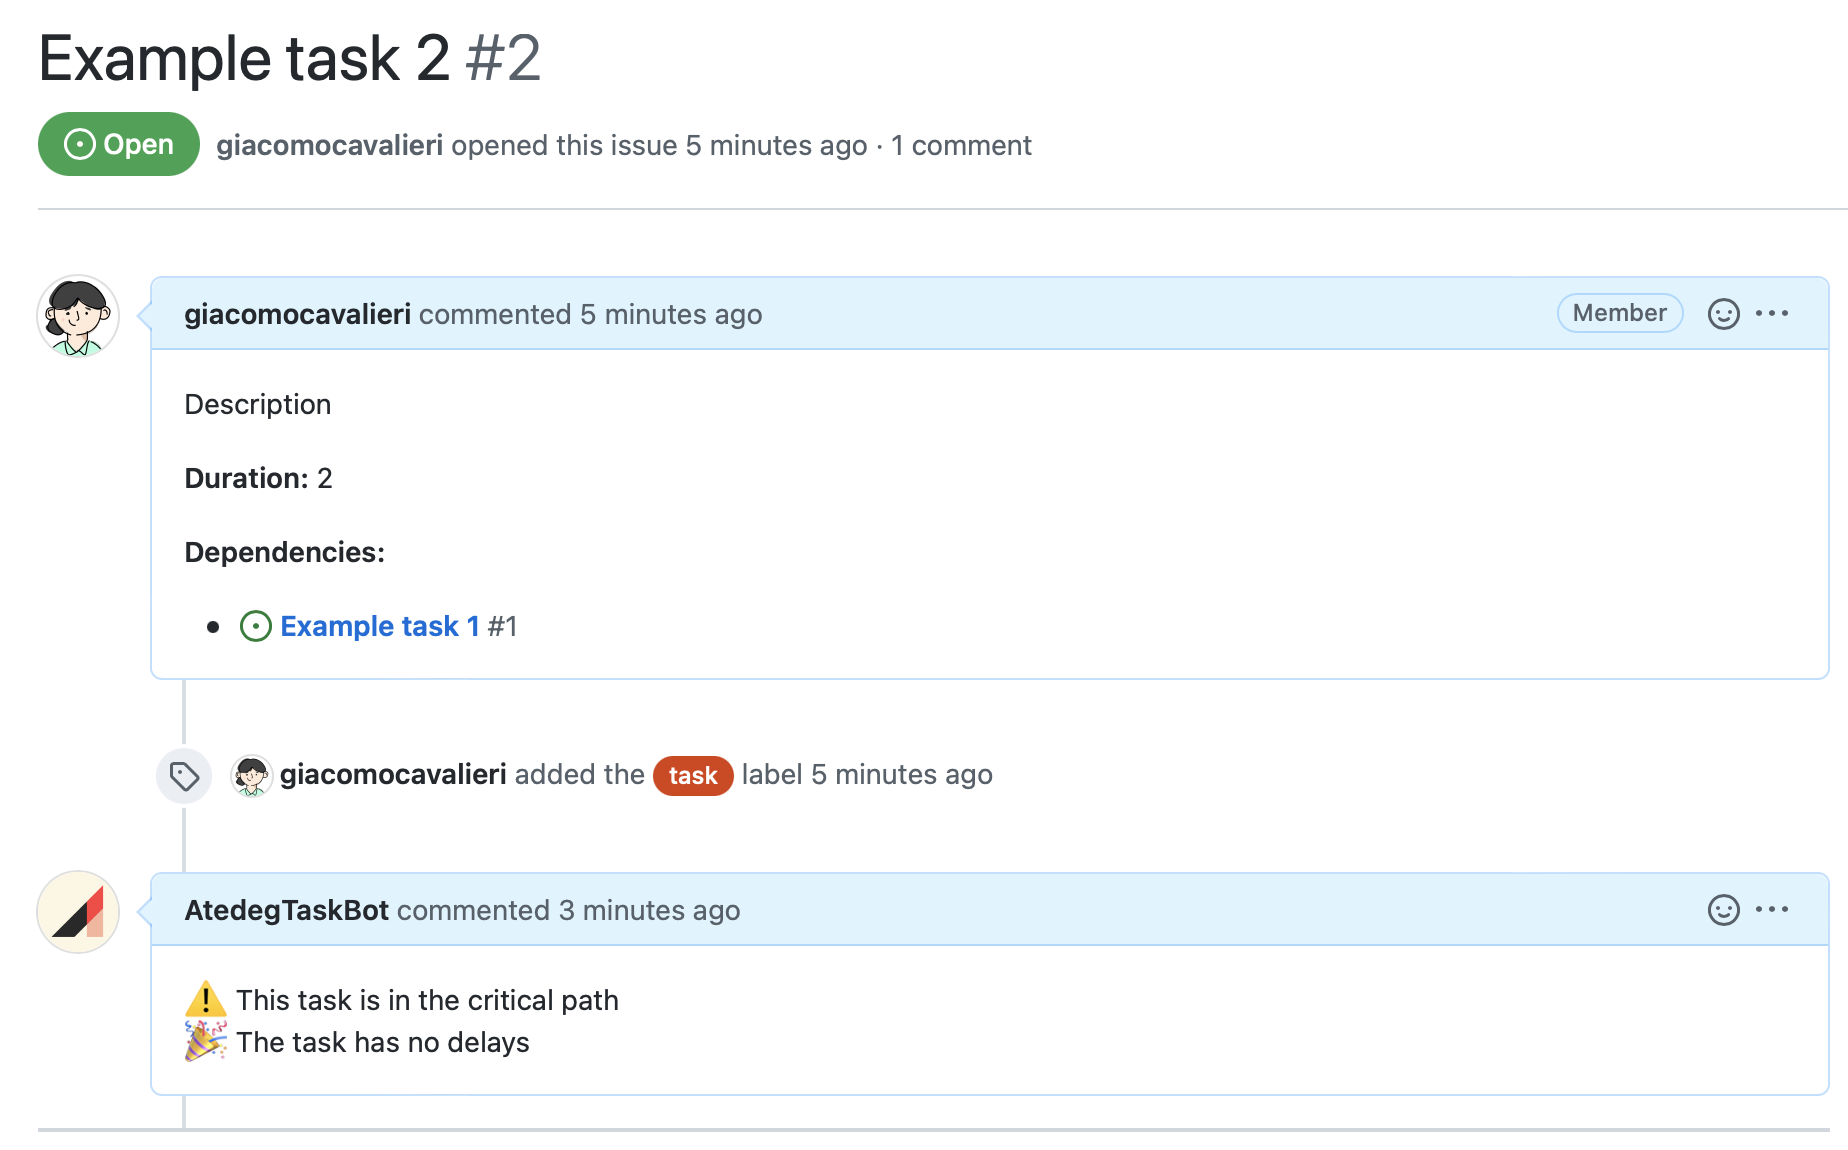
\includegraphics[width=\textwidth]{images/task-example.png}
  \caption{Esempio di issue}
  \label{fig:issue-example}
\end{figure}

\subsection{Sprint burndown chart}
Inoltre, ad ogni sprint viene generato automaticamente uno \emph{sprint burndown chart} a partire dalle issue chiuse. Questo grafico viene aggiornato al completamento dei task e permette di monitorare lo stato di avanzamento dello sprint in tempo reale.
È uno strumento fondamentale che permette di individuare rapidamente dei ritardi sulla tabella di marcia permettendo al team di analizzarne le cause tempestivamente.

Come mostrato in \Cref{fig:sprint-burndown-chart}, il grafico riporta sull'asse delle ascisse il giorno dello sprint e sull'asse delle ordinate l'effort rimanente. Inflessioni del grafico indicano ritardi o avanzamenti rispetto alla tabella di marcia ideale.

\begin{figure}
\centering
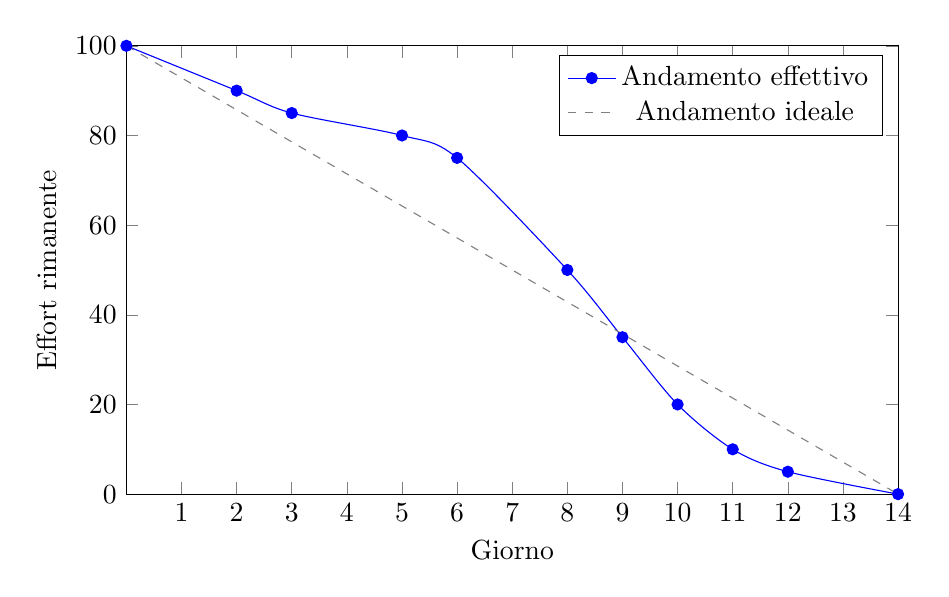
\begin{tikzpicture}
  \begin{axis}[
      xlabel={Giorno},
      ylabel={Effort rimanente},
      xmin=0, xmax=14,
      x=0.7cm,
      ymin=0, ymax=100,
      xtick={1,...,14},
      ytick={0,20,...,100}]
  \addplot[smooth,mark=*,blue] plot coordinates {
      (0,100)
      (2,90)
      (3,85)
      (5,80)
      (6,75)
      (8,50)
      (9,35)
      (10,20)
      (11,10)
      (12,5)
      (14,0)
  };
  \addlegendentry{Andamento effettivo}
  
  \addplot[dashed,color=gray,mark=none]
      plot coordinates {
          (0,100)
          (14,0)
      };
  \addlegendentry{Andamento ideale}
  \end{axis}
\end{tikzpicture}
\caption{Esempio di sprint burndown chart}
\label{fig:sprint-burndown-chart}
\end{figure}

\subsection{Project Burndown Chart}
È stato anche realizzato un \emph{project burndown chart} che mostra lo stato di avanzamento del progetto. 
Anche in questo caso il grafico viene generato automaticamente a partire dalle issue chiuse e permette di monitorare l'intero progetto.
Come mostrato in \Cref{fig:project-burndown-chart}, il grafico riporta gli sprint sull'asse delle ascisse e il numero di story point rimanenti sull'asse delle ordinate.

Questo strumento è fondamentale per poter stimare la velocità di sviluppo del team nel consumare story points. Infatti, per stimare il numero di story points da realizzare in uno sprint devono essere tenute in considerazione le storie concluse in precedenza ed eventuali difficoltà del team nel portarle a compimento.
Così facendo è possibile mantenere una velocità di sviluppo all'incirca costante per poter stimare con maggior precisione le tempistiche di consegna del progetto.

\begin{figure}
  \centering
  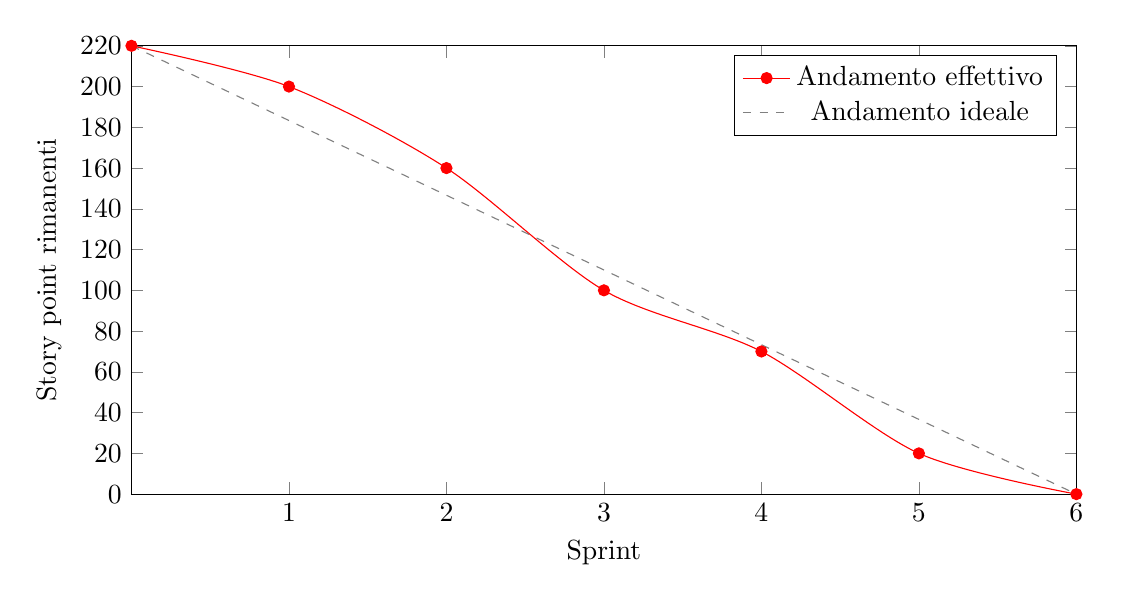
\begin{tikzpicture}
    \begin{axis}[
        xlabel={Sprint},
        ylabel={Story point rimanenti},
        xmin=0, xmax=6,
        x=2cm,
        ymin=0, ymax=220,
        xtick={1,...,6},
        ytick={0,20,...,220}]
    \addplot[smooth,mark=*,red] plot coordinates {
        (0,220)
        (1,200)
        (2,160)
        (3,100)
        (4,70)
        (5,20)
        (6,0)
    };
    \addlegendentry{Andamento effettivo}
    
    \addplot[dashed,color=gray,mark=none]
        plot coordinates {
            (0,220)
            (6,0)
        };
    \addlegendentry{Andamento ideale}
    \end{axis}
  \end{tikzpicture}
  \caption{Esempio di project burndown chart}
  \label{fig:project-burndown-chart}
  \end{figure}



\todo[inline]{Mettere il network diagram all'inizio di ogni sprint}
\todo[inline]{FARE LO SPRINT BURNDOWN CHART}

\appendix
\chapter{Cartellone dell'event storming}
\label{app:cartellone-event-storming}

\begin{figure}[!ht]
  \centering
  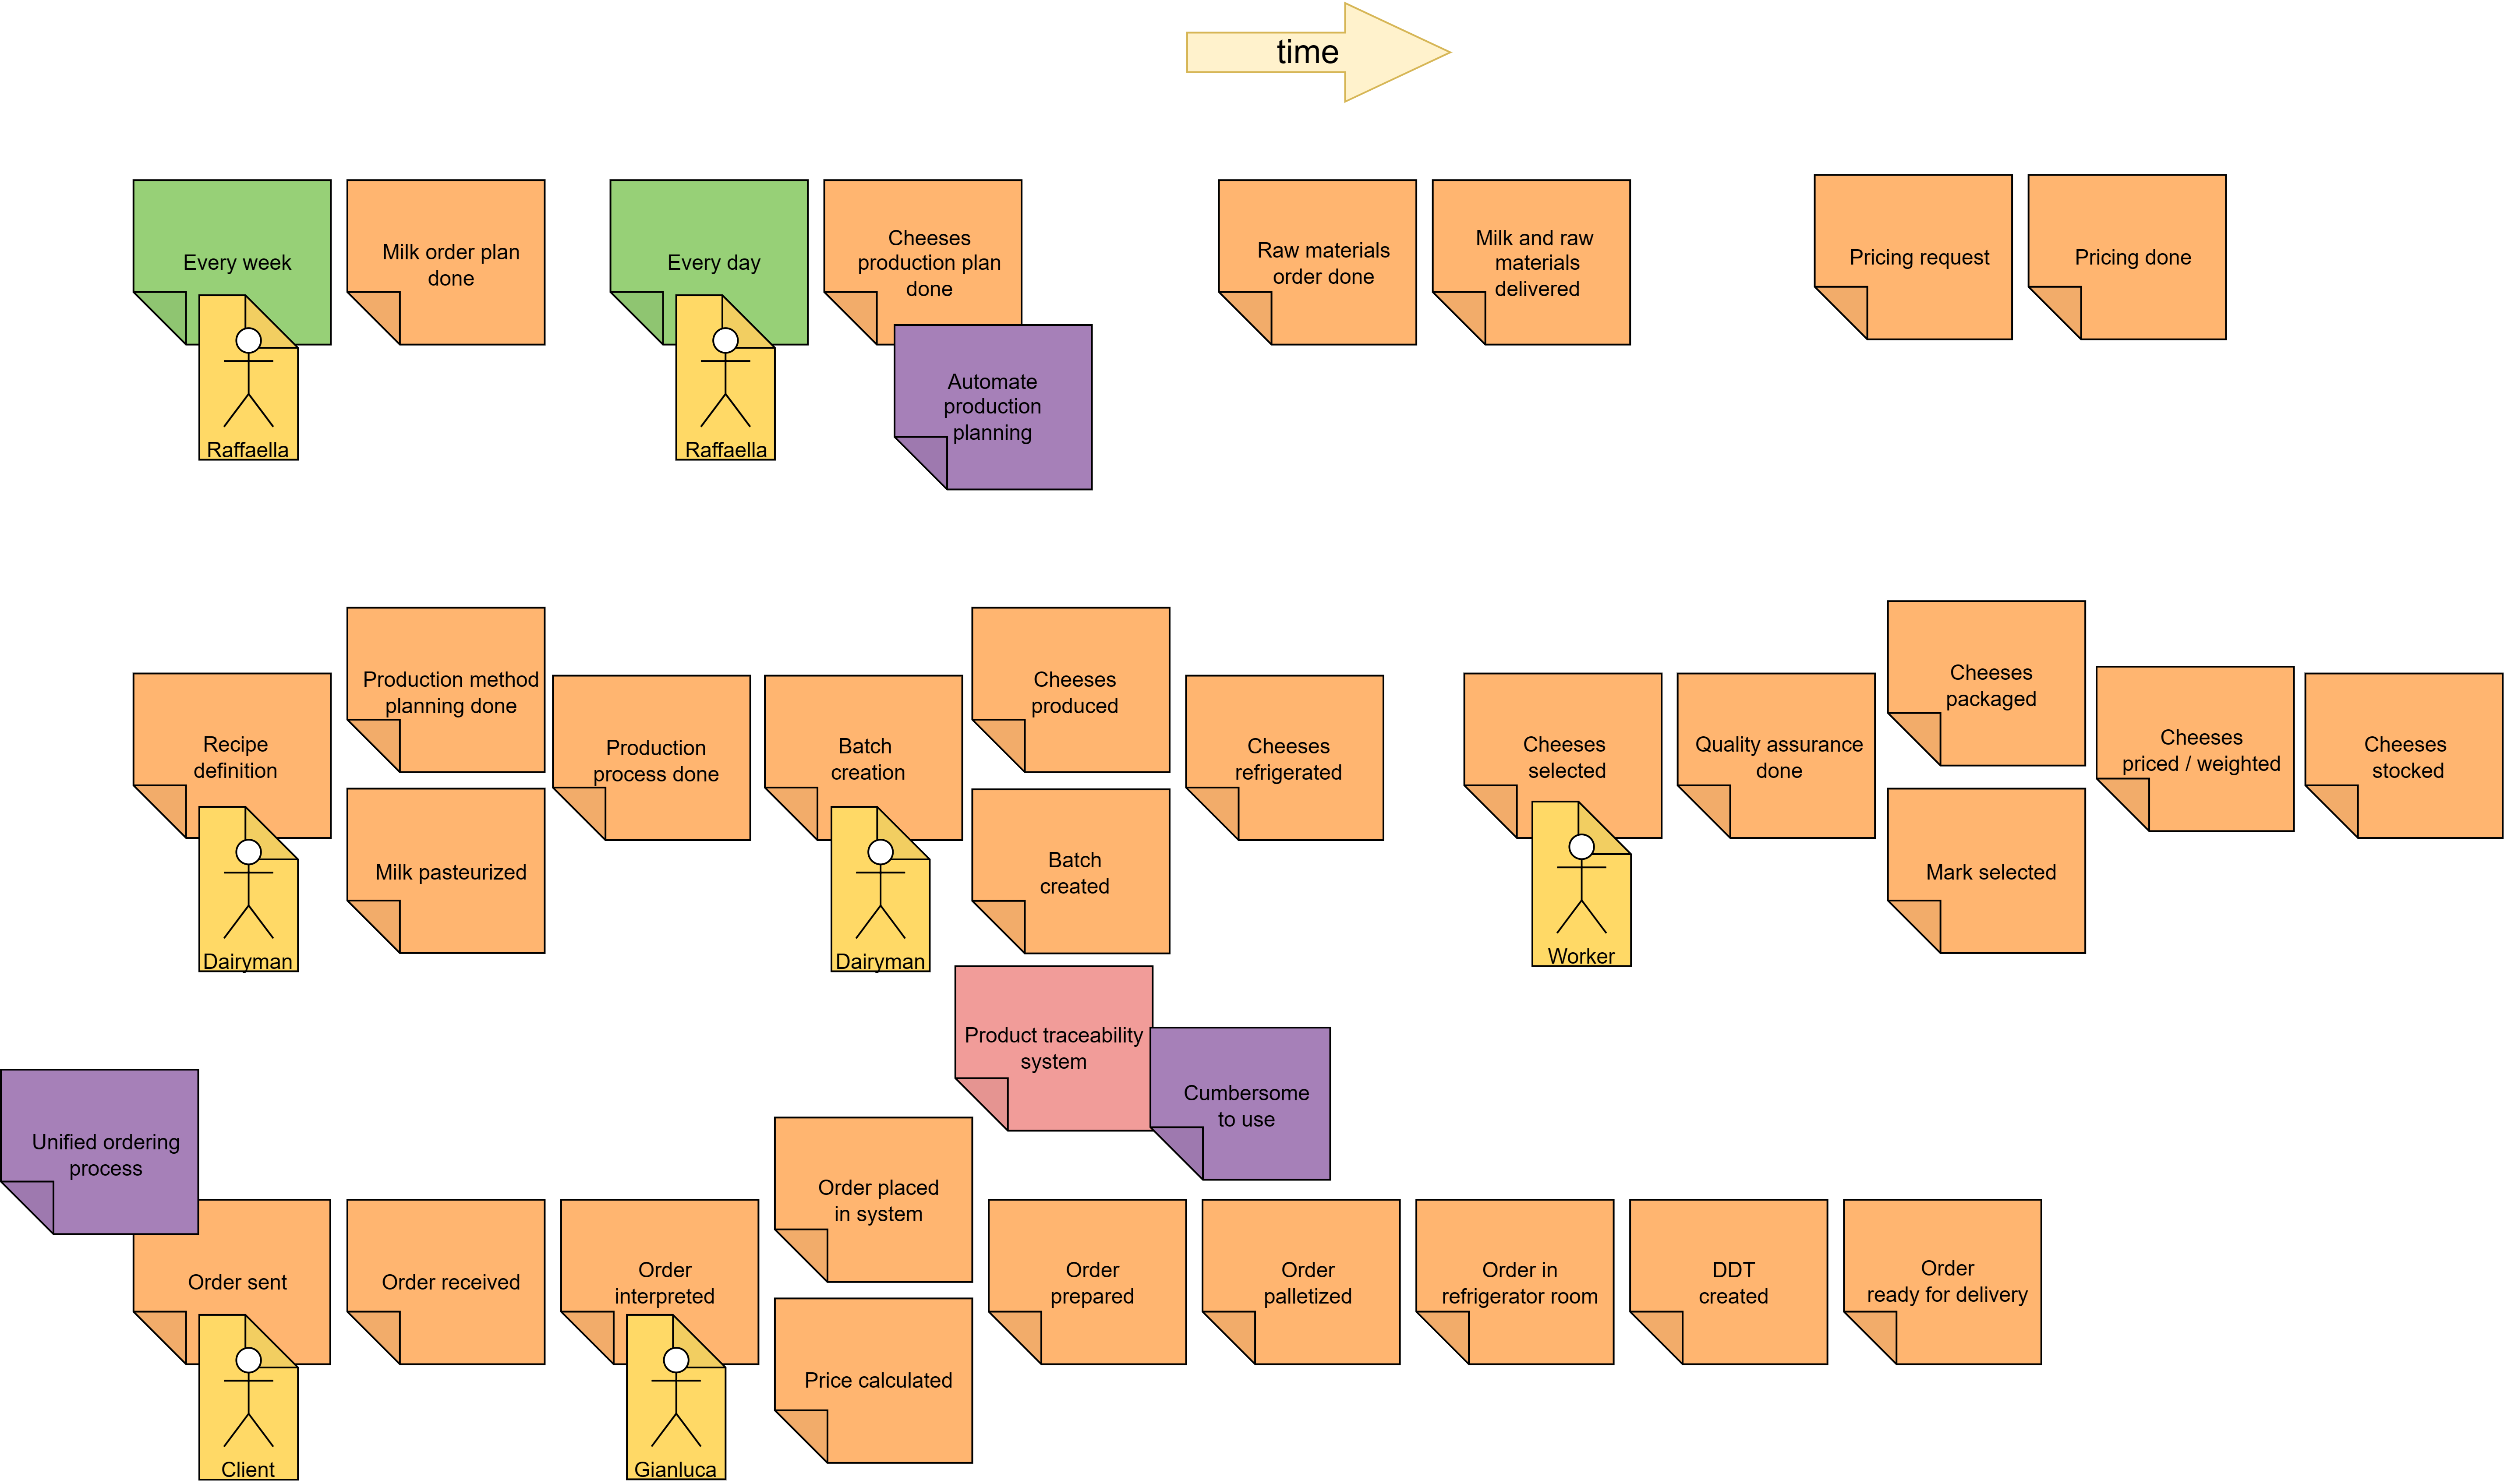
\includegraphics[width=0.8\textwidth]{images/event-storming.png}
  \caption{Risultato finale ottenuto con l'event storming}
  \label{fig:event-storming-result}
\end{figure}
\chapter{Cartellone con evidenziati i bounded context}
\label{app:cartellone-event-storming-bc}

\begin{figure}[!ht]
  \centering
  \includegraphics[width=.8\textwidth]{images/event-storming-bc.png}
  \caption{Suddivisione in bounded context}
  \label{fig:seconda-riunione-bc}
\end{figure}
\chapter{Ubiquitous Language}
\label{app:ubiquitous-language}

\section{Definizioni condivise}
\begin{description}
    \item[Tipo di formaggio] La tipologia di un formaggio prodotto.
    \item[Prodotto] Un tipo di formaggio con il suo rispettivo peso.
    \item[Ingrediente] Un ingrediente necessario per produrre un tipo di formaggio.
\end{description}

\section{Pianificazione del riordino del latte}
\begin{description}
    \item [Latte processato] I quintali di latte processati per poter produrre dei formaggi.
    \item [Quintali di latte] Una quantità di latte espressa in quintali.
    \item [Resa] Un decimale che rappresenta la resa del latte nella produzione di un determinato tipo di formaggio: \textit{i.e.} per produrre $n$ quintali di un certo formaggio con una resa $r$ servono $r \cdot n$ quintali di latte.
    \item [Ricettario] Definisce, per ogni tipologia di formaggio, la resa del latte nella sua produzione.
    \item [Scorta] Definisce, per ogni prodotto, la quantità in magazzino.
    \item [Quantità in magazzino] La quantità di un prodotto in magazzino, potrebbe anche essere 0.
    \item [Quantità] La quantità di qualcosa.
    \item [Prodotto richiesto] Un prodotto richiesto in una certa quantità che deve essere pronto entro una certa data.
\end{description}

\section{Pianificazione della produzione}
\begin{description}
    \item [Piano di produzione] Tutti i prodotti che devono essere prodotti in un giorno.
    \item [Prodotto da produrre] Un formaggio che deve essere prodotto in una data quantità.
    \item [Prodotto mancante] Un prodotto con il numero di unità mancanti che devono essere aggiunte al magazzino.
    \item [Ordine] Un insieme di prodotti ordinati e una data entro la quale l'ordine deve essere completato.
    \item [Prodotto ordinato] Un prodotto richiesto in una certa quantità.
    \item [Giorni di stagionatura] i giorni di invecchiamento in cella che devono passare per un formaggio prima che questo sia pronto.
\end{description}

\section{Produzione}
\begin{description}
    \item [Piano di produzione] Si compone di linee che specificano cosa produrre.
    \item [Linea del piano di produzione] Una linea di un piano di produzione che specifica un prodotto e quante unità di esso produrre.
    \item [Produzione da avviare] Una produzione che deve essere avviata specifica il prodotto da produrre e in che quantità deve essere prodotto.
    \item [Produzione avviata] Una produzione che deve essere avviata specifica il prodotto in produzione e in che quantità deve essere prodotto.
    \item [Produzione conclusa] Una produzione che è stata conclusa, ha un ID che ne identifica il lotto e specifica il prodotto e in che quantità è stato prodotto.
    \item [Ricettario] Associa ad ogni tipo di formaggio una ricetta.
    \item [Ricetta] Una lista di ingredienti e i rispettivi quintali necessari per produrre un quintale di un prodotto.
    \item [Quintali di ingrediente] Un ingrediente e un peso in quintali.
    \item [Giorni di stagionatura] I giorni di invecchiamento in cella che devono passare per un formaggio prima che questo sia pronto.
\end{description}

\section{Magazzino}
\begin{description}
    \item [Scorte disponibili] I prodotti attualmente disponibili in magazzino; ogni prodotto è disponibile in una certa quantità (che può anche essere zero se il prodotto è esaurito).
    \item [Scorte desiderate] La quantità desiderata di ogni prodotto che deve essere sempre presente in magazzino per avere un certo margine di sicurezza per la gestione delle consegne.
    \item [Quantità disponibile] La quantità di un prodotto disponibile in magazzino.
    \item [Quantità desiderata] La quantità desiderata di un prodotto che dovrebbe essere presente in magazzino.
    \item [Quantità mancante] La quantità di un prodotto mancante per raggiungere il livello di stock desiderato.
    \item [Lotto] Un lotto di prodotti di un certo tipo, identificato da un ID, che non è stato ancora sottoposto a controllo di qualità.
    \item [Lotto certificato] Un lotto di prodotti di un certo tipo, identificato da un ID, che è stato sottoposto a controllo di qualità.
    \item [Prodotto etichettato] Un prodotto con la sua quantità e l'ID del lotto a cui appartiene.
\end{description}

\section{Rifornimento}
\begin{description}
    \item[Scorte] Definisce per ogni ingrediente la quantità disponibile in magazzino.
    \item[Latte in magazzino] Quintali di latte in magazzino.
    \item[Quintali di ingrediente] Un ingrediente e un peso in quintali.
    \item[Quintali di latte] Una quantità di latte espressa in quintali.
\end{description}

\section{Ordini dei clienti}
\begin{description}
    \item[Ordine in arrivo]
    Un insieme di linee d'ordine con le rispettive quantità (ad esempio 1000 ricotte di 0,5 kg, 50 squacqueroni di 1 kg), contiene anche dati sul cliente, una data di consegna prevista e il luogo di consegna.
    \item[Linea di un ordine in arrivo] Un prodotto con la quantità ordinata.
    \item[Cliente] Un'entità fisica o giuridica che piazza gli ordini.
    \item[Luogo] Il luogo dove un ordine deve essere spedito.
    \item[Ordine prezzato] Un ordine dove ogni linea ha un prezzo associato e, opzionalmente, uno sconto applicato. Ha anche un prezzo totale. La sua struttura è simile a quella dell'ordine in arrivo con la differenza che ogni linea è stata prezzata.
    \item[Linea di un ordine prezzato] Un prodotto con la sua quantità e un prezzo.
    \item[Ordine in elaborazione] Un ordine che sta venendo elaborato da un operatore. La sua struttura è simile a quella dell'ordine prezzato con la differenza che ogni linea può specificare se è stata completata o meno.
    \item[Linea di un ordine in elaborazione] Un prodotto con la sua quantità, un prezzo e lo stato di completamento. Può essere in due stati: completa se il prodotto è già stato palletizzato e è pronto nella quantità richiesta; incompleta se il prodotto non è presente nella quantità richiesta.
    \item[Ordine completato] Un ordine che è stato completato da un operatore ed è pronto per essere spedito.
    \item[Linea di un ordine completato] Un prodotto con la sua quantità e un prezzo.
    \item[DDT] Un documento che deve specificare: il luogo di consegna, il luogo di spedizione, i dati del cliente, la data di spedizione, il peso totale del pallet e un insieme di linee del DDT.
    \item[Linea del DDT] Un prodotto con la sua quantità spedita.
\end{description}

\section{Prezzatura}
\begin{description}
    \item[Linea d'ordine in arrivo] Un prodotto con la sua quantità ordinata.
    \item[Quantità] Una quantità di qualcosa.
    \item[Listino] Associa a ogni prodotto il suo prezzo unitario.
    \item[Prezzo] Un prezzo espresso in centesimi d'euro.
    \item[Client] Un'entità fisica o giuridica che piazza gli ordini.
    \item[ID Cliente] Un ID che identifica in maniera univoca un cliente.
    \item[Promozione] Una promozione per un cliente, con una data di scadenza, che contiene delle linee di promozione per alcuni prodotti.
    \item[Linea di promozione fissa] Questa linea di promozione specifica il prodotto scontato e di quanto scontarlo. Ogni linea d'ordine che contiene il prodotto è scontata di quanto specificato.
    \item[Linea di promozione a soglia] Questa linea di promozione specifica il prodotto scontato, la soglia e di quanto scontarlo. Solo ordinati in quantità superiore alla soglia sono scontati; gli altri sono a prezzo pieno.
    \item[Soglia] Una quantità che indica il numero minimo di prodotti da ordinare perché uno sconto possa essere applicato.
    \item[Percentuale di sconto] Una percentuale di sconto espressa con un numero compreso fra 0 (escluso) e 100 (incluso).
\end{description}
\chapter{User Stories}
\label{app:user-stories}
In seguito sono riportate le user stories definite in accordo con il committente. Le user stories sono state organizzate in iniziative (I) ed epiche (E).
Ciascuna iniziativa fa riferimento ad un diverso bounded context e si compone di epiche e user stories; ciascuna user story è identificata da una sigla che indica l'iniziativa -- ed eventualmente l'epica -- a cui fa riferimento. Per esempio ``I1-E1-U2'' indica la seconda user story dell'epica E1 dell'iniziativa I1.

\section*{I1: Pianificazione della produzione}

\begin{table}[H]
  \begin{tabularx}{\textwidth}{lX}
    \toprule
    \textbf{I1-E1} & \textbf{Generazione del piano di produzione} \\
    \midrule
    \textbf{In quanto} & Raffaella \\
    \textbf{vorrei} & generare automaticamente un piano di produzione per il giorno \\
    \textbf{così da} & ottimizzare l'utilizzo delle macchine per la produzione di formaggio durante la giornata \\
    \midrule
    \textbf{CoS} & Il piano di produzione è adeguato per soddisfare tutti gli ordini in tempo \\
    & Le macchine sono inattive per al massimo il 15\% del tempo \\
    \midrule
    \textbf{Priorità} & 3 \\
    \bottomrule
  \end{tabularx}
  \label{user-story:i1-e1}
\end{table}

\begin{table}[H]
  \begin{tabularx}{\textwidth}{lX}
    \toprule
    \textbf{I1-E1-U1} & \textbf{Soddisfazione degli ordini nel piano di produzione generato} \\
    \midrule
    \textbf{In quanto} & Raffaella \\
    \textbf{vorrei} & verificare che il piano di produzione generato soddisfi tutti gli ordini \\
    \textbf{così da} & assicurarmi che tutti gli ordini possano essere evasi \\
    \midrule
    \textbf{CoS} & Il piano di produzione generato include la produzione di tutte le unità richieste dagli ordini nei tempi prescritti \\
    \midrule
    \textbf{Priorità} & 5 \\
    \textbf{Story points} & 20 \\
    \textbf{N. persone} & 2 \\
    \bottomrule
  \end{tabularx}
  \label{user-story:i1-e1-u1}
\end{table}

\begin{table}[H]
  \begin{tabularx}{\textwidth}{lX}
    \toprule
    \textbf{I1-E1-U2} & \textbf{Ottimizzazione dell'utilizzo delle macchine} \\
    \midrule
    \textbf{In quanto} & Raffaella \\
    \textbf{vorrei} & limitare il tempo di inattività delle macchine per la produzione di formaggio al 15\% o meno \\
    \textbf{così da} & ottenere il massimo rendimento dall'utilizzo delle macchine \\
    \midrule
    \textbf{CoS} & Il piano di produzione generato include solo il tempo necessario per la produzione e le macchine sono inattive per al massimo il 15\% del tempo \\
    \midrule
    \textbf{Priorità} & 3 \\
    \textbf{Story points} & 20 \\
    \textbf{N. persone} & 2 \\
    \bottomrule
  \end{tabularx}
  \label{user-story:i1-e1-u2}
\end{table}

\begin{table}[H]
  \begin{tabularx}{\textwidth}{lX}
    \toprule
    \textbf{I1-E2} & \textbf{Visualizzazione del piano di produzione} \\
    \midrule
    \textbf{In quanto} & Raffaella \\
    \textbf{vorrei} & visualizzare il piano di produzione attuale \\
    \textbf{così da} & conoscere ciò che è stato generato \\
    \midrule
    \textbf{CoS} & L'interfaccia è facile da usare e comprendere secondo le Euristiche di Nielsen~\cite{cit:nielsen} \\
    \midrule
    \textbf{Priorità} & 4 \\
    \bottomrule
  \end{tabularx}
  \label{user-story:i1-e2}
\end{table}

\begin{table}[H]
  \begin{tabularx}{\textwidth}{lX}
    \toprule
    \textbf{I1-E2-U1} & \textbf{Visualizzazione del volume di produzione pianificato} \\
    \midrule
    \textbf{In quanto} & Raffaella \\
    \textbf{vorrei} & visualizzare il numero di unità pianificate per ogni prodotto \\
    \textbf{così da} & conoscere il volume di produzione previsto \\
    \midrule
    \textbf{CoS} & L'interfaccia presenta una tabella con le informazioni sulla pianificazione delle unità di produzione per ogni prodotto \\
    \midrule
    \textbf{Priorità} & 5 \\
    \textbf{Story points} & 1 \\
    \textbf{N. persone} & 1 \\
    \bottomrule
  \end{tabularx}
  \label{user-story:i1-e2-u1}
\end{table}

\begin{table}[H]
  \begin{tabularx}{\textwidth}{lX}
    \toprule
    \textbf{I1-E2-U2} & \textbf{Visualizzazione del volume di produzione effettivo} \\
    \midrule
    \textbf{In quanto} & Raffaella \\
    \textbf{vorrei} & visualizzare il numero di unità effettivamente prodotte per ogni prodotto \\
    \textbf{così da} & confrontare il volume di produzione previsto con quello effettivo \\
    \midrule
    \textbf{CoS} & L'interfaccia presenta una tabella con le informazioni sulla produzione effettiva per ogni prodotto \\
    \midrule
    \textbf{Priorità} & 3 \\
    \textbf{Story points} & 1 \\
    \textbf{N. persone} & 1 \\
    \bottomrule
  \end{tabularx}
  \label{user-story:i1-e2-u2}
\end{table}

\begin{table}[H]
  \begin{tabularx}{\textwidth}{lX}
    \toprule
    \textbf{I1-E2-U3} & \textbf{Filtro nella visualizzazione del piano di produzione} \\
    \midrule
    \textbf{In quanto} & Raffaella \\
    \textbf{vorrei} & filtrare la visualizzazione del piano di produzione in base alla data di pianificazione o di produzione \\
    \textbf{così da} & analizzare il piano di produzione in un determinato periodo di tempo \\
    \midrule
    \textbf{CoS} & L'interfaccia presenta opzioni di filtraggio per la data di pianificazione o di produzione \\
    \midrule
    \textbf{Priorità} & 1 \\
    \textbf{Story points} & 3 \\
    \textbf{N. persone} & 1 \\
    \bottomrule
  \end{tabularx}
  \label{user-story:i1-e2-u3}
\end{table}

\begin{table}[H]
  \begin{tabularx}{\textwidth}{lX}
    \toprule
    \textbf{I1-U1} & \textbf{Modifica del piano di produzione} \\
    \midrule
    \textbf{In quanto} & Raffaella \\
    \textbf{vorrei} & modificare il piano di produzione generato per il giorno \\
    \textbf{così da} & tenere conto di situazioni eccezionali che potrebbero verificarsi durante la giornata \\
    \midrule
    \textbf{CoS} & Il piano di produzione può essere modificato prima di essere approvato per la produzione \\
    \midrule
    \textbf{Priorità} & 5 \\
    \textbf{Story points} & 5 \\
    \textbf{N. persone} & 1 \\
    \bottomrule
  \end{tabularx}
  \label{user-story:i1-u1}
\end{table}

\section*{I2: Ordini dei clienti}

\begin{table}[H]
  \begin{tabularx}{\textwidth}{lX}
    \toprule
    \textbf{I2-U1} & \textbf{Prezzatura automatica} \\
    \midrule
    \textbf{In quanto} & magazziniere \\
    \textbf{vorrei} & che il sistema calcolasse automaticamente i prezzi degli ordini in entrata \\
    \textbf{così da} & evitare di doverlo fare manualmente sfogliando l'elenco dei prezzi \\
    \midrule
    \textbf{CoS} & Il sistema calcola automaticamente i prezzi degli ordini in entrata utilizzando una versione digitale del listino prezzi attualmente in uso \\
    \midrule
    \textbf{Priorità} & 3 \\
    \textbf{Story points} & 4 \\
    \textbf{N. persone} & 1 \\
    \bottomrule
  \end{tabularx}
  \label{user-story:i2-u1}
\end{table}

\begin{table}[H]
  \begin{tabularx}{\textwidth}{lX}
    \toprule
    \textbf{I2-E1} & \textbf{Pallettizzazione automatica} \\
    \midrule
    \textbf{In quanto} & magazziniere \\
    \textbf{vorrei} & pallettizzare un prodotto per un ordine \\
    \textbf{così da} & poter mettere da parte un prodotto per l'ordine di un cliente \\
    \midrule
    \textbf{CoS} & Il magazziniere può scansionare il codice a barre del prodotto con un palmare per contrassegnarlo come pallettizzato e aggiornare le forniture del magazzino \\
    \midrule
    \textbf{Priorità} & 4 \\
    \bottomrule
  \end{tabularx}
  \label{user-story:i2-e1}
\end{table}

\begin{table}[H]
  \begin{tabularx}{\textwidth}{lX}
    \toprule
    \textbf{I2-E1-U1} & \textbf{Contrassegnare il prodotto come pallettizzato} \\
    \midrule
    \textbf{In quanto} & magazziniere \\
    \textbf{vorrei} & contrassegnare il prodotto come pallettizzato \\
    \textbf{così da} & aggiornare le informazioni del magazzino e preparare il prodotto per l'ordine di un cliente \\
    \midrule
    \textbf{CoS} & È possibile interagire con il sistema segnalando la pallettizzazione di un prodotto \\
    \midrule
    \textbf{Priorità} & 5 \\
    \textbf{Story points} & 6 \\
    \textbf{N. persone} & 1 \\
    \bottomrule
  \end{tabularx}
  \label{user-story:i2-e1-u1}
\end{table}

\begin{table}[H]
  \begin{tabularx}{\textwidth}{lX}
    \toprule
    \textbf{I2-E1-U2} & \textbf{Scansione dei prodotti con un palmare} \\
    \midrule
    \textbf{In quanto} & magazziniere \\
    \textbf{vorrei} & contrassegnare il prodotto come pallettizzato scansionandone il codice a barre tramite un palmare \\
    \textbf{così da} & non dover inserire manualmente il codice del prodotto \\
    \midrule
    \textbf{CoS} & L'interfaccia del palmare permette di scansionare il codice a barre del prodotto e contrassegnarlo come pallettizzato \\
    \midrule
    \textbf{Priorità} & 4 \\
    \textbf{Story points} & 6 \\
    \textbf{N. persone} & 1 \\
    \bottomrule
  \end{tabularx}
  \label{user-story:i2-e1-u2}
\end{table}

\begin{table}[H]
  \begin{tabularx}{\textwidth}{lX}
    \toprule
    \textbf{I2-E1-U3} & \textbf{Aggiornamento delle forniture del magazzino} \\
    \midrule
    \textbf{In quanto} & magazziniere \\
    \textbf{vorrei} & aggiornare le forniture del magazzino quando un prodotto viene pallettizzato \\
    \textbf{così da} & tenere traccia della quantità di prodotto disponibile nel magazzino \\
    \midrule
    \textbf{CoS} & Quando un prodotto viene contrassegnato come pallettizzato, le informazioni del magazzino vengono aggiornate di conseguenza \\
    \midrule
    \textbf{Priorità} & 3 \\
    \textbf{Story points} & 5 \\
    \textbf{N. persone} & 1 \\
    \bottomrule
  \end{tabularx}
  \label{user-story:i2-e1-u3}
\end{table}

\begin{table}[H]
  \begin{tabularx}{\textwidth}{lX}
    \toprule
    \textbf{I2-E1-U4} & \textbf{Integrazione con il sistema di tracciabilità} \\
    \midrule
    \textbf{In quanto} & magazziniere \\
    \textbf{vorrei} & aggiungere automaticamente le informazioni del prodotto al sistema di tracciabilità quando lo pallettizzo per un ordine \\
    \textbf{così da} & evitare di doverlo fare manualmente \\
    \midrule
    \textbf{CoS} & Il sistema aggiunge automaticamente le informazioni del prodotto al sistema di tracciabilità quando viene scansionato il suo codice per aggiungerlo a un ordine \\
    \midrule
    \textbf{Priorità} & 5 \\
    \textbf{Story points} & 15 \\
    \textbf{N. persone} & 3 \\
    \bottomrule
  \end{tabularx}
  \label{user-story:i2-e1-u4}
\end{table}

\begin{table}[H]
  \begin{tabularx}{\textwidth}{lX}
    \toprule
    \textbf{I2-E2} & \textbf{Completare un ordine} \\
    \midrule
    \textbf{In quanto} & magazziniere \\
    \textbf{vorrei} & poter segnare un ordine come completo e pronto per essere spedito \\
    \textbf{così da} & poterlo spedire al cliente \\
    \midrule
    \textbf{CoS} & L'operatore può segnare un ordine come completo sfruttando un palmare \\
    \midrule
    \textbf{Priorità} & 3 \\
    \bottomrule
  \end{tabularx}
  \label{user-story:i2-e2}
\end{table}

\begin{table}[H]
  \begin{tabularx}{\textwidth}{lX}
    \toprule
    \textbf{I2-E2-U1} & \textbf{Segnare un ordine come completo} \\
    \midrule
    \textbf{In quanto} & magazziniere \\
    \textbf{vorrei} & avere la possibilità di segnare un ordine come completo \\
    \textbf{così da} & poterlo preparare per la spedizione al cliente \\
    \midrule
    \textbf{CoS} & È possibile interagire con il sistema per segnare un ordine come completo \\
    \midrule
    \textbf{Priorità} & 5 \\
    \textbf{Story points} & 7 \\
    \textbf{N. persone} & 1 \\
    \bottomrule
  \end{tabularx}
  \label{user-story:i2-e2-u1}
\end{table}

\begin{table}[H]
  \begin{tabularx}{\textwidth}{lX}
    \toprule
    \textbf{I2-E2-U2} & \textbf{Uso del palmare per segnare un ordine come completo} \\
    \midrule
    \textbf{In quanto} & magazziniere \\
    \textbf{vorrei} & utilizzare un palmare per segnare un ordine come completo \\
    \textbf{così da} & non dover inserire manualmente il codice dell'ordine per segnarlo come completo\\
    \midrule
    \textbf{CoS} & L'interfaccia del palmare permette di scansionare il codice dell'ordine per segnarlo come completo \\
    \midrule
    \textbf{Priorità} & 4 \\
    \textbf{Story points} & 6 \\
    \textbf{N. persone} & 1 \\
    \bottomrule
  \end{tabularx}
  \label{user-story:i2-e2-u2}
\end{table}

\begin{table}[H]
  \begin{tabularx}{\textwidth}{lX}
    \toprule
    \textbf{I2-E3} & \textbf{Generazione e stampa del DDT} \\
    \midrule
    \textbf{In quanto} & magazziniere \\
    \textbf{vorrei} & generare automaticamente un DDT per un ordine che è pronto per essere spedito \\
    \textbf{così da} & non doverlo fare manualmente \\
    \midrule
    \textbf{CoS} & Il sistema raccoglie automaticamente informazioni sui prodotti contenuti nel pallet dell'ordine e permette di stampare il DDT scansionando l'ID del pallet con un tablet \\
    \midrule
    \textbf{Priorità} & 2 \\
    \bottomrule
  \end{tabularx}
  \label{user-story:i2-e3}
\end{table}

\begin{table}[H]
  \begin{tabularx}{\textwidth}{lX}
    \toprule
    \textbf{I2-E3-U1} & \textbf{Generazione automatica del DDT} \\
    \midrule
    \textbf{In quanto} & magazziniere \\
    \textbf{vorrei} & generare automaticamente un DDT per un ordine pronto per la spedizione \\
    \textbf{così da} & evitare il processo manuale di compilazione del DDT \\
    \midrule
    \textbf{CoS} & Il sistema raccoglie automaticamente informazioni sui prodotti contenuti nell'ordine e permette di generare il DDT automaticamente \\
    \midrule
    \textbf{Priorità} & 5 \\
    \textbf{Story points} & 8 \\
    \textbf{N. persone} & 2 \\
    \bottomrule
  \end{tabularx}
  \label{user-story:i2-e3-u1}
\end{table}

\begin{table}[H]
  \begin{tabularx}{\textwidth}{lX}
    \toprule
    \textbf{I2-E3-U2} & \textbf{Utilizzo di un tablet per stampare il DDT} \\
    \midrule
    \textbf{In quanto} & magazziniere \\
    \textbf{vorrei} & utilizzare un tablet per stampare il DDT generato automaticamente per un ordine \\
    \textbf{così da} & non dover inserire manualmente il codice dell'ordine per stamparne il DDT \\
    \midrule
    \textbf{CoS} & L'interfaccia del tablet permette di mandare in stampa il DDT generato automaticamente scansionando l'ID del pallet dell'ordine \\
    \midrule
    \textbf{Priorità} & 3 \\
    \textbf{Story points} & 6 \\
    \textbf{N. persone} & 1 \\
    \bottomrule
  \end{tabularx}
  \label{user-story:i2-e3-u2}
\end{table}

\begin{table}[H]
  \begin{tabularx}{\textwidth}{lX}
    \toprule
    \textbf{I2-E4} & \textbf{Piazzamento ordini online} \\
    \midrule
    \textbf{In quanto} & cliente \\
    \textbf{vorrei} & poter sfruttare un portale di e-commerce per poter fare i miei acquisti \\
    \textbf{così da} & scegliere ed acquistare i prodotti che mi servono \\
    \midrule
    \textbf{CoS} & C'è un sito web che permette di scegliere quali prodotti acquistare tramite un catalogo e offre la possibilità di scegliere diverse metodologie di pagamento \\
    \midrule
    \textbf{Priorità} & 5 \\
    \bottomrule
  \end{tabularx}
  \label{user-story:i2-e4}
\end{table}

\begin{table}[H]
  \begin{tabularx}{\textwidth}{lX}
    \toprule
    \textbf{I2-E4-U1} & \textbf{Creazione sito web di Mambelli} \\
    \midrule
    \textbf{In quanto} & cliente \\
    \textbf{vorrei} & poter consultare il sito web del caseificio \\
    \textbf{così da} & avere un unico portale da consultare al bisogno \\
    \midrule
    \textbf{CoS} & C'è un sito web minimale del caseificio \\ 
    \midrule
    \textbf{Priorità} & 5 \\
    \textbf{Story points} & 20 \\
    \textbf{N. persone} & 4-5 \\
    \bottomrule
  \end{tabularx}
  \label{user-story:i2-e4-u1}
\end{table}

\begin{table}[H]
  \begin{tabularx}{\textwidth}{lX}
    \toprule
    \textbf{I2-E4-U2} & \textbf{Grafica del sito web} \\
    \midrule
    \textbf{In quanto} & Raffaella \\
    \textbf{vorrei} & che il nuovo sito mantenesse una grafica simile al precedente sito vetrina utilizzato dal caseificio \\
    \textbf{così da} & mantenere uno stile coerente riconoscibile dai clienti \\
    \midrule
    \textbf{CoS} & Il nuovo sito realizzato riprende il linguaggio visuale adottato dal precedente sito vetrina \\ 
    \midrule
    \textbf{Priorità} & 1 \\
    \textbf{Story points} & 7 \\
    \textbf{N. persone} & 1 \\
    \bottomrule
  \end{tabularx}
  \label{user-story:i2-e4-u2}
\end{table}

\begin{table}[H]
  \begin{tabularx}{\textwidth}{lX}
    \toprule
    \textbf{I2-E4-U3} & \textbf{Digitalizzazione del catalogo Mambelli} \\
    \midrule
    \textbf{In quanto} & Raffaella \\
    \textbf{vorrei} & una versione digitale dell'attuale catalogo di Mambelli \\
    \textbf{così da} & poter gestire con più facilità il catalogo dei prodotti del caseificio \\
    \midrule
    \textbf{CoS} & Il catalogo è salvato in una base di dati \\
    \midrule
    \textbf{Priorità} & 4 \\
    \textbf{Story points} & 2 \\
    \textbf{N. persone} & 1 \\
    \bottomrule
  \end{tabularx}
  \label{user-story:i2-e4-u3}
\end{table}

\begin{table}[H]
  \begin{tabularx}{\textwidth}{lX}
    \toprule
    \textbf{I2-E4-U4} & \textbf{Modifica del catalogo Mambelli} \\
    \midrule
    \textbf{In quanto} & Raffaella \\
    \textbf{vorrei} & poter modificare il catalogo dei prodotti \\
    \textbf{così da} & poter aggiornare le descrizioni dei prodotti del caseificio o aggiungerne di nuovi qualora necessario \\
    \midrule
    \textbf{CoS} & C'è una semplice interfaccia che permette a Raffaella di modificare il catalogo memorizzato \\
    \midrule
    \textbf{Priorità} & 2 \\
    \textbf{Story points} & 5 \\
    \textbf{N. persone} & 1 \\
    \bottomrule
  \end{tabularx}
  \label{user-story:i2-e4-u4}
\end{table}

\begin{table}[H]
  \begin{tabularx}{\textwidth}{lX}
    \toprule
    \textbf{I2-E4-U5} & \textbf{Visualizzazione del catalogo online} \\
    \midrule
    \textbf{In quanto} & cliente \\
    \textbf{vorrei} & sfogliare un catalogo online di tutti i prodotti disponibili \\
    \textbf{così da} & scegliere cosa comprare \\
    \midrule
    \textbf{CoS} & È possibile consultare nel sito web il catalogo di tutti i prodotti che possono essere acquistati presso il caseificio \\
    \midrule
    \textbf{Priorità} & 5 \\
    \textbf{Story points} & 3 \\
    \textbf{N. persone} & 1 \\
    \bottomrule
  \end{tabularx}
  \label{user-story:i2-e4-u5}
\end{table}

\begin{table}[H]
  \begin{tabularx}{\textwidth}{lX}
    \toprule
    \textbf{I2-E4-U6} & \textbf{Carrello per gli acquisti online} \\
    \midrule
    \textbf{In quanto} & cliente \\
    \textbf{vorrei} & mettere i formaggi a cui sono interessato in un carrello \\
    \textbf{così da} & poterli ordinare online \\
    \midrule
    \textbf{CoS} & Il sito web permette di mettere i prodotti in un carrello per poterli poi ordinare \\
    \midrule
    \textbf{Priorità} & 5 \\
    \textbf{Story points} & 7 \\
    \textbf{N. persone} & 1 \\
    \bottomrule
  \end{tabularx}
  \label{user-story:i2-e4-u6}
\end{table}

\begin{table}[H]
  \begin{tabularx}{\textwidth}{lX}
    \toprule
    \textbf{I2-E4-U7} & \textbf{Ordini online} \\
    \midrule
    \textbf{In quanto} & cliente \\
    \textbf{vorrei} & poter fare un ordine con tutti i miei prodotti messi nel carrello \\
    \textbf{così da} & comprare i formaggi di cui ho bisogno \\
    \midrule
    \textbf{CoS} & C'è un pulsante per effettuare l'acquisto dei prodotti che ho messo nel carrello \\
    \midrule
    \textbf{Priorità} & 5 \\
    \textbf{Story points} & 12 \\
    \textbf{N. persone} & 3 \\
    \bottomrule
  \end{tabularx}
  \label{user-story:i2-e4-u7}
\end{table}

\begin{table}[H]
  \begin{tabularx}{\textwidth}{lX}
    \toprule
    \textbf{I2-E4-U8} & \textbf{Metodi di pagamento} \\
    \midrule
    \textbf{In quanto} & cliente \\
    \textbf{vorrei} & poter scegliere fra più metodologie di pagamento \\
    \textbf{così da} & scegliere quella che mi conviene di più \\
    \midrule
    \textbf{CoS} & Un cliente può scegliere di pagare con un bonifico, in contanti alla consegna oppure tramite carta di credito \\
    \midrule
    \textbf{Priorità} & 5 \\
    \textbf{Story points} & 15 \\
    \textbf{N. persone} & 3 \\
    \bottomrule
  \end{tabularx}
  \label{user-story:i2-e4-u8}
\end{table}

\begin{table}[H]
  \begin{tabularx}{\textwidth}{lX}
    \toprule
    \textbf{I2-E4-U9} & \textbf{Unificazione dell'e-commerce e del sito vetrina} \\
    \midrule
    \textbf{In quanto} & cliente \\
    \textbf{vorrei} & un unico sito con informazioni sul caseificio e l'e-commerce \\
    \textbf{così da} & non dover cambiare sito per piazzare i miei ordini una volta aver consultato la vetrina \\
    \midrule
    \textbf{CoS} & Il sito web realizzato per l'e-commerce contiene anche varie informazioni sul caseificio \\ 
    \midrule
    \textbf{Priorità} & 3 \\
    \textbf{Story points} & 5 \\
    \textbf{N. persone} & 1 \\
    \bottomrule
  \end{tabularx}
  \label{user-story:i2-e4-u9}
\end{table}

\begin{table}[H]
  \begin{tabularx}{\textwidth}{lX}
    \toprule
    \textbf{I2-E4-U10} & \textbf{Sito web sempre disponibile} \\
    \midrule
    \textbf{In quanto} & Raffaella \\
    \textbf{vorrei} & che il sito fosse sempre raggiungibile senza disservizi \\
    \textbf{così da} & non spingere i clienti verso la concorrenza se dovessero trovare il sito offline \\
    \midrule
    \textbf{CoS} & L'infrastruttura è sufficiente a gestire il flusso di clienti del caseificio \\
    & Il sito web è disponibile nel 99\% del tempo in un anno \\
    \midrule
    \textbf{Priorità} & 4 \\
    \textbf{Story points} & 10 \\
    \textbf{N. persone} & 2 \\
    \bottomrule
  \end{tabularx}
  \label{user-story:i2-e4-u10}
\end{table}

\begin{table}[H]
  \begin{tabularx}{\textwidth}{lX}
    \toprule
    \textbf{I2-E4-U11} & \textbf{User experience del sito} \\
    \midrule
    \textbf{In quanto} & cliente \\
    \textbf{vorrei} & che il sito fosse facile da utilizzare \\
    \textbf{così da} & poter effettuare gli ordini senza difficoltà \\
    \midrule
    \textbf{CoS} & Il sito rispetta le Euristiche di Nielsen \\
    & Almeno il 90\% degli utenti finali che hanno testato i mockup del sito lo hanno valutato positivamente \\
    \midrule
    \textbf{Priorità} & 3 \\
    \textbf{Story points} & 13 \\
    \textbf{N. persone} & 2 \\
    \bottomrule
  \end{tabularx}
  \label{user-story:i2-e4-u11}
\end{table}

\section*{I3: Gestione del magazzino}

\begin{table}[H]
  \begin{tabularx}{\textwidth}{lX}
    \toprule
    \textbf{I3-U1} & \textbf{Tracciamento automatico della disponibilità dei prodotti} \\
    \midrule
    \textbf{In quanto} & magazziniere \\
    \textbf{vorrei} & che il sistema tenga traccia automaticamente della disponibilità dei prodotti \\
    \textbf{così da} & non doverlo fare manualmente \\
    \midrule
    \textbf{CoS} & Il sistema tiene automaticamente traccia delle disponibilità di ciascun prodotto e le aggiorna mano a mano che i prodotti vengono tolti dal magazzino per essere spediti ai clienti \\
    \midrule
    \textbf{Priorità} & 3 \\
    \textbf{Story points} & 5 \\
    \textbf{N. persone} & 1 \\
    \bottomrule
  \end{tabularx}
  \label{user-story:i3-u1}
\end{table}


\begin{table}[H]
  \begin{tabularx}{\textwidth}{lX}
    \toprule
    \textbf{I3-U2} & \textbf{Visualizzazione della disponibilità dei prodotti} \\
    \midrule
    \textbf{In quanto} & magazziniere \\
    \textbf{vorrei} & avere la possibilità di visualizzare la disponibilità di ciascun prodotto \\
    \textbf{così da} & sapere quali prodotti sono disponibili \\
    \midrule
    \textbf{CoS} & L'interfaccia permette di visualizzare la disponibilità di ciascun prodotto in tempo reale \\
    \midrule
    \textbf{Priorità} & 3 \\
    \textbf{Story points} & 3 \\
    \textbf{N. persone} & 1 \\
    \bottomrule
  \end{tabularx}
  \label{user-story:i3-u2}
\end{table}

\chapter{Project Overview Statement}
\label{app:pos}

\section{Problems/Opportunities}
L'azienda ha riscontrato un grande aumento nel volume degli ordini, rendendo difficile gestirli con un processo manuale come sempre fatto fino ad ora.
Per questo motivo ha bisogno di un sistema che permetta di raccogliere e gestire in maniera efficiente gli ordini dei clienti; questo sistema deve essere realizzato categoricamente entro il 30 settembre per poter essere sfruttato nella gestione del flusso di ordini del periodo natalizio. Inoltre, l'azienda necessita di un sistema che permetta di automatizzare la pianificazione della produzione dei prodotti per aumentare l'efficienza nell'uso dei macchinari. Infatti, con una pianificazione manuale si è osservato come ci siano fasce orarie in cui i macchinari non sono utilizzati.
Infine, è importante che il nuovo sistema di gestione degli ordini si integri automaticamente con il sistema della tracciabilità adottato dall'azienda.

\section{Goals}
\begin{itemize}
  \item Unificazione dei canali per l'acquisto dei prodotti da parte dei clienti entro settembre
  \item Centralizzazione della gestione degli ordini e della loro tracciabilità
  \item Automazione della pianificazione della produzione per massimizzare la produttività dei macchinari
\end{itemize}

\section{Objectives}
\begin{itemize}
  \item Realizzazione di un portale web per permettere ai clienti di piazzare ordini
  \item Realizzazione di un sistema che permetta di gestire automaticamente il ciclo di vita degli ordini
  \item Integrazione del sistema degli ordini con il sistema della tracciabilità preesistente
  \item Realizzazione di un sistema che permetta di pianificare automaticamente la produzione giornaliera
\end{itemize}

\section{Success Criteria}
\begin{itemize}
  \item Il portale web viene utilizzato per effettuare almeno il 90\% degli ordini
  \item Il sistema di pianificazione della produzione deve realizzare un piano entro dieci minuti dal momento della richiesta
  \item Il piano generato automaticamente deve permettere di soddisfare il 95\% degli ordini ricevuti
  \item Il piano generato automaticamente deve far in modo che i macchinari siano sempre utilizzati al massimo della loro capacità
  \item Non è necessario alcun intervento manuale aggiuntivo per gestire la tracciabilità dei prodotti negli ordini dei clienti
\end{itemize}

\section{Assumptions}
\begin{itemize}
  \item Il cliente può sostenere i costi dovuti alla realizzazione dell'intero progetto
  \item Il cliente dispone di dati storici sulla pianificazione della produzione
  \item I palmari a disposizione dei magazzinieri sono sufficientemente moderni per potersi connettere a internet
\end{itemize}

\section{Risks}
\begin{itemize}
  \item I clienti abituati a contattare direttamente l'azienda per effettuare gli ordini potrebbero non adeguarsi al nuovo sistema
  \item La normativa europea sui documenti di trasporto potrebbe cambiare durante la realizzazione del progetto
  \item L'integrazione con il sistema della tracciabilità potrebbe non essere possibile o molto laboriosa
  \item Il cliente potrebbe aggiungere una nuova linea di prodotti durante lo sviluppo del sistema
  \item Potrebbe non essere possibile effettuare la consegna del sito di e-commerce con la gestione degli ordini entro il 30 settembre
  \item I dati storici relativi alla pianificazione della produzione potrebbero essere di qualità insufficiente per realizzare in maniera efficace un sistema di pianificazione automatica
  \item Potrebbero non essere disponibili utenti finali del sistema per effettuare le prove di usabilità tramite focus group
\end{itemize}

\section{Obstacles}
\begin{itemize}
  \item Il sistema di gestione degli ordini deve essere pronto entro settembre per poter essere utilizzato per la stagione invernale
  \item Alcuni membri del team non hanno esperienza di DDD e richiedono lezioni di formazione
\end{itemize}


\chapter{Analisi dei rischi}
\label{app:analisi-rischi}

\begin{table}[H]
  \begin{tabularx}{\textwidth}{lX}
    \toprule
    \textbf{Rischio}            & \textbf{I clienti abituati a contattare direttamente l'azienda per effettuare gli ordini potrebbero non adeguarsi al nuovo sistema}                                                \\
    \midrule
    \textbf{Probabilità}        & Probabile                                                                                                                                                                          \\
    \textbf{Impatto}            & Critico                                                                                                                                                                            \\
    \textbf{Livello di rischio} & Alto                                                                                                                                                                               \\
    \textbf{Mitigazione}        & Grande attenzione alla user experience del prodotto realizzato sfruttando anche focus group in modo da assicurarsi che i clienti possano adattarsi facilmente alla nuova soluzione \\
                                & Campagna di promozione per incentivare l'adozione del nuovo sistema per esempio con degli sconti                                                                                   \\
    \bottomrule
  \end{tabularx}
\end{table}

\begin{table}[H]
  \begin{tabularx}{\textwidth}{lX}
    \toprule
    \textbf{Rischio}            & \textbf{La normativa europea sui documenti di trasporto potrebbe cambiare durante la realizzazione del progetto}                      \\
    \midrule
    \textbf{Probabilità}        & Possibile                                                                                                                             \\
    \textbf{Impatto}            & Critico                                                                                                                               \\
    \textbf{Livello di rischio} & Alto                                                                                                                                  \\
    \textbf{Mitigazione}        & Analizzare la proposta di legge per individuare quali porzioni del sistema sarebbero interessate in modo da anticipare il cambiamento \\
    \bottomrule
  \end{tabularx}
\end{table}

\begin{table}[H]
  \begin{tabularx}{\textwidth}{lX}
    \toprule
    \textbf{Rischio}            & \textbf{L'integrazione con il sistema della tracciabilità potrebbe non essere possibile}                                                                      \\
    \midrule
    \textbf{Probabilità}        & Improbabile                                                                                                                                                   \\
    \textbf{Impatto}            & Catastrofico                                                                                                                                                  \\
    \textbf{Livello di rischio} & Alto                                                                                                                                                          \\
    \textbf{Mitigazione}        & Verificare prima di accettare il progetto che sia effettivamente possibile interagire (tramite un'API o altre tecnologie) con il servizio della tracciabilità \\
    \bottomrule
  \end{tabularx}
\end{table}

\begin{table}[H]
  \begin{tabularx}{\textwidth}{lX}
    \toprule
    \textbf{Rischio}            & \textbf{L'integrazione con il sistema della tracciabilità potrebbe richiedere più tempo del previsto} \\
    \midrule
    \textbf{Probabilità}        & Possibile                                                                                             \\
    \textbf{Impatto}            & Marginale                                                                                             \\
    \textbf{Livello di rischio} & Medio                                                                                                 \\
    \textbf{Mitigazione}        & Dedicare più risorse all'integrazione durante lo sprint in cui verrà svolto                           \\
    \bottomrule
  \end{tabularx}
\end{table}

\begin{table}[H]
  \begin{tabularx}{\textwidth}{lX}
    \toprule
    \textbf{Rischio}            & \textbf{Il cliente potrebbe aggiungere una nuova linea di prodotti durante lo sviluppo del sistema}     \\
    \midrule
    \textbf{Probabilità}        & Possibile                                                                                               \\
    \textbf{Impatto}            & Marginale                                                                                               \\
    \textbf{Livello di rischio} & Medio                                                                                                   \\
    \textbf{Mitigazione}        & Rendere il sistema flessibile in modo da poter supportare l'aggiunta di nuovi prodotti in corso d'opera \\
    \bottomrule
  \end{tabularx}
\end{table}

\begin{table}[H]
  \begin{tabularx}{\textwidth}{lX}
    \toprule
    \textbf{Rischio}            & \textbf{Potrebbe non essere possibile effettuare la consegna del sito di e-commerce con la gestione degli ordini entro il 30 settembre} \\
    \midrule
    \textbf{Probabilità}        & Improbabile                                                                                                                             \\
    \textbf{Impatto}            & Catastrofico                                                                                                                            \\
    \textbf{Livello di rischio} & Alto                                                                                                                                    \\
    \textbf{Mitigazione}        & Dare massima priorità alla realizzazione dell'e-commerce                                                                                \\
                                & Realizzare subito una prima interfaccia minimale da far validare al cliente                                                             \\
                                & Risparmiare tempo riutilizzando componenti già sviluppati in precedenza per altri progetti                                              \\
    \bottomrule
  \end{tabularx}
\end{table}

\begin{table}[H]
  \begin{tabularx}{\textwidth}{lX}
    \toprule
    \textbf{Rischio}            & \textbf{I dati storici relativi alla pianificazione della produzione potrebbero essere di qualità insufficiente per realizzare in maniera efficace un sistema di pianificazione automatica} \\
    \midrule
    \textbf{Probabilità}        & Possibile                                                                                                                                                                                   \\
    \textbf{Impatto}            & Critico                                                                                                                                                                                     \\
    \textbf{Livello di rischio} & Alto                                                                                                                                                                                        \\
    \textbf{Mitigazione}        & Prima di accettare il progetto verificare la presenza di dati per la pianificazione automatica                                                                                              \\
                                & Se non presenti, si potrebbe rimandare la pianificazione automatica a un secondo momento e avviare un processo di raccolta dei dati storici sulla pianificazione nel formato più adatto     \\
    \bottomrule
  \end{tabularx}
\end{table}

\begin{table}[H]
  \begin{tabularx}{\textwidth}{lX}
    \toprule
    \textbf{Rischio}            & \textbf{Nicolas prenderà parte alla conferenza \href{https://zfoh.ch/zurihac2022/}{ZuriHack} dal 11 giugno al 13 giugno} \\
    \midrule
    \textbf{Probabilità}        & Certo                                                                                                                    \\
    \textbf{Impatto}            & Minore                                                                                                                   \\
    \textbf{Livello di rischio} & Alto                                                                                                                     \\
    \textbf{Mitigazione}        & Ridurre il numero di user story nello sprint interessato                                                                 \\
    \bottomrule
  \end{tabularx}
\end{table}

\begin{table}[H]
  \begin{tabularx}{\textwidth}{lX}
    \toprule
    \textbf{Rischio}            & \textbf{Sviluppatori potrebbero essere irreperibili per via di situazioni eccezionali (malattia, infortuni, ecc.)}                                                                                                                       \\
    \midrule
    \textbf{Probabilità}        & Possibile                                                                                                                                                                                                                                \\
    \textbf{Impatto}            & Critico                                                                                                                                                                                                                                  \\
    \textbf{Livello di rischio} & Alto                                                                                                                                                                                                                                     \\
    \textbf{Mitigazione}        & In caso di assenze prolungate si può considerare l'assunzione di nuovo personale a progetto                                                                                                                                              \\
                                & La schedula degli sprint viene fatta in modo da non occupare tutti gli sviluppatori al 100\%; viene lasciato un certo slack in modo che sia possibile per uno sviluppatore coprire -- anche solo parzialmente -- l'assenza di un collega \\
                                & Rimodulazione dello sprint backlog per adattare il carico di lavoro agli sviluppatori rimanenti                                                                                                                                          \\
    \bottomrule
  \end{tabularx}
\end{table}

\begin{table}[H]
  \begin{tabularx}{\textwidth}{lX}
    \toprule
    \textbf{Rischio}            & \textbf{Potrebbero non essere disponibili utenti finali del sistema per effettuare le prove di usabilità tramite focus group}                                              \\
    \midrule
    \textbf{Probabilità}        & Improbabile                                                                                                                                                                \\
    \textbf{Impatto}            & Marginale                                                                                                                                                                  \\
    \textbf{Livello di rischio} & Medio                                                                                                                                                                      \\
    \textbf{Mitigazione}        & Fin da subito iniziare a prendere contatti con i possibili clienti in modo da ricevere il prima possibile le loro disponibilità e organizzare i focus group in tempi utili \\
                                & Fornire un incentivo economico alla partecipazione ai focus group (per esempio sotto forma di sconto sulle merci ordinate)                                                 \\
                                & Utilizzo di componenti grafiche standard e di qualità per avere una buona baseline di usabilità                                                                            \\
    \bottomrule
  \end{tabularx}
\end{table}

\chapter{Sprint backlog del terzo sprint}
In seguito è riportato un elenco che mostra le storie pianificate per il terzo sprint con la relativa scomposizione in task e loro stime

\begin{itemize}
  \item \href{}{I2-E4-U2}: Grafica del sito web
        \begin{itemize}
          \item Ottenere i vecchi fogli di stile adottati dal caseificio (effort 1)
          \item Adattare il vecchio stile al nuovo sito (effort 4)
        \end{itemize}
  \item \href{}{I2-E4-U4}: Modifica del catalogo Mambelli
        \begin{itemize}
          \item Definire lo schema del DB (effort 4)
          \item Definire interfaccia per comunicare con il database (effort 3)
          \item Implementare query per aggiornare il database (effort 2)
          \item Realizzare form per poter permettere all'utente di modificare il database (effort 2)
        \end{itemize}
  \item \href{}{I2-E4-U9}: Unificazione dell'e-commerce e del sito vetrina
        \begin{itemize}
          \item Realizzare un mockup del risultato finale (effort 11)
          \item Richiedere la validazione del cliente del mockup (effort 3)
          \item Integrare il mockup nel sito effettivo (effort 7)
          \item Integrare gli stili adottati per il sito effettivo (effort 5)
        \end{itemize}
  \item \href{}{I2-E4-U3}: Digitalizzazione del catalogo Mambelli
        \begin{itemize}
          \item Ottenere il precedente catalogo (effort 1)
          \item Stabilire uno schema per il database dove immagazzinarlo (effort 4)
          \item Implementare il database (effort 5)
        \end{itemize}
  \item \href{}{I1-E1-U1}: Soddisfazione degli ordini nel piano di produzione generato
        \begin{itemize}
          \item Raccogliere i dati forniti dal committente (effort 2)
          \item Analisi dei dati (effort 10)
          \item Pulizia dei dati (effort 5)
          \item Definire i criteri di valutazione (effort 2)
          \item Definizione di un modello (effort 7)
          \item Training del modello (effort 3)
          \item Valutazione delle prestazioni del modello (effort 4)
          \item Messa in produzione (effort 3)
        \end{itemize}
  \item \href{}{I1-E2-U1}: Visualizzazione del volume di produzione pianificato
        \begin{itemize}
          \item Definizione dell'interfaccia che il risultato del modello deve seguire (effort 2)
          \item Realizzare un mockup del risultato finale (effort 4)
          \item Richiedere la validazione del cliente del mockup (effort 3)
          \item Integrare il mockup nell'applicativo per la pianificazione (effort 6)
        \end{itemize}
  \item \href{}{I1-E2-U2}: Visualizzazione del volume di produzione effettivo
        \begin{itemize}
          \item Realizzare un mockup del risultato finale (effort 4)
          \item Richiedere la validazione del cliente del mockup (effort 3)
          \item Integrare il mockup nell'applicativo per la pianificazione (effort 6)
        \end{itemize}
  \item \href{}{I1-E2-U3}: Filtro nella visualizzazione del piano di produzione
        \begin{itemize}
          \item Realizzare un mockup del risultato finale (effort 4)
          \item Richiedere la validazione del cliente del mockup (effort 3)
          \item Integrare il mockup nell'applicativo per la pianificazione (effort 6)
        \end{itemize}
  \item \href{}{I1-U1}: Modifica del piano di produzione
        \begin{itemize}
          \item Stabilire le modalità con cui interagire con il piano di produzione realizzato (effort 3)
          \item Implementare le query di modifica del piano (effort 2)
          \item Integrazione nell'interfaccia utente della possibilità di modificare il piano (effort 5)
        \end{itemize}
\end{itemize}

\printbibliography[title={Riferimenti Bibliografici}]
\end{document}